\chapter{Search strategy}
\label{chap:analysis}

This chapter describes the analysis strategy of a search for physics 
beyond the standard model in proton-proton collisions at a centre of mass 
energy of 13~TeV. The search is performed in final states containing missing 
transverse momentum and at least one jet. 

The search is designed to have sensitivity to a wide range of new physics 
models that involve the production of a weakly interacting 
particle (WIMP), such as dark matter or the lightest supersymmetric particle. 
The search has been optimised for signatures in which the WIMP is produced from 
prompt decays at the primary collision vertex. However, as will be discussed in 
Chap.~\ref{chap:results}, the search is also sensitive to signatures in which 
the WIMP is produced at a displaced vertex following the decay of a long-lived 
particle. %This will be the focus of the interpretation.
% OB: prompt MET signatures

%explain hard scatter somewhere?
% overall momentum
%is an imbalance in transverse momentum in the final state, as they travel 
%through the detector without interacting %undetected
% this whole paragraph might need to go somewhere else (maybe intro or chap2)
In the proton-proton collisions, the net momentum of the colliding partons in 
the plane transverse to the beam direction is effectively zero, whereas the 
longitudinal momentum is not necessarily so. In order to conserve momentum, the 
outgoing particles produced in the collision must therefore have an overall 
transverse momentum of zero. As WIMPs do not interact with the detector 
material, the measured net transverse momentum in the event will be non-zero. 
This non-zero ``missing transverse momentum'' is the key signature of such 
particles. In addition, at a hadron collider such as the LHC, the dominant 
production is via the strong interaction, and hence jets are readily produced 
either in association with the WIMP, or as initial or final state radiation 
(ISR, FSR). For these two reasons the search is performed in final states 
containing jets and missing energy. The requirement of at least one jet is 
needed for the missing momentum to be defined and for the event to be 
triggered. A hadronic final state is ensured by vetoing events containing 
leptons or photons.

A missing energy signature is not unique to WIMPs, however, and is also present 
in certain standard model processes. Neutrinos (produced in the decays of Z and 
W bosons, for example) are also weakly interacting and undetectable at CMS. It 
is also possible for particles to be over or under-measured, thereby 
introducing a ``fake'' momentum imbalance. This type of background arising from 
energy mismeasurements is suppressed as much as possible (to lt1\% of the total 
background) using the variables described in Sec.~X. The remaining standard 
model background (that involving neutrinos) must be estimated as precisely as 
possible, using a combination of theory calculations, simulation, and 
calibrations in data. This is described in Sec.~X. One can then look for a 
statistically significant excess in the data above the expected amount of 
standard model background that would be an indication of the observation of 
physics beyond the standard model. The statistical analysis is covered in 
Chap.~\ref{chap:results}.

In order to maximise the sensitivity to a wide range of SUSY and DM scenarios, 
all of which may manifest themselves in topologically slightly different ways 
in the detector, the candidate signal events (which form part of the 
\textit{signal region}) are categorised according to four variables (the total 
jet energy, the missing jet energy, the number of jets, and the number of 
b-tagged jets) as detailed 
in Sec.~X. Two \textit{control regions} are defined, labelled \mj and 
\mmj, that are analogous to the signal region but are enriched by 
selection of muons in the W and Z background processes, respectively, and are 
employed in the background estimations as described in Sec.~X.
%inclusiveness
%The ways in which a WIMP/BSM signature can manifest are numerous

Similar searches for supersymmetry have been performed in Runs 1 and 2 of the 
LHC, at centre of mass energies of 8 and 13~TeV, and for a range of 
integrated luminosities. These can be found in Refs.~[1,2,3,4,5]. These 
searches are used as a basis for the analysis described in this thesis. A 
series of developments and optimisations have been made in order to adapt the 
analysis for the higher centre of mass energy and larger amount of data 
collected. In addition, the interpretations in dark matter and long-lived 
particles described in Chap.~X are a novelty to this search.

%has ptmiss been defined?

%This chapter is organised as follows: Section bla describes bla etc.
% just mention as you go along

\begin{comment}
Variable definitions, trigger, selections, binning, signal and control regions, 
background estimations, systematic uncertainties, likelihood model

See AN and paper (old ones too) and theses

This search does not employ specialized reconstruction techniques [36–41] that 
target long-lived gluinos



Inclusive, jets + MET search for new physics
(lots of params in susy)
►Low thresholds of HT > 200 GeV, MHT > 130 GeV, Njet >= 1
►Maximise sensitivity by binning in Njet, Nb, HT, MHT ►Using dedicated 
variables αT, Δφ* to strongly suppress the QCD background ►Data-driven 
estimation of EWK and QCD backgrounds using several control regions

Intro/overview (1-2 pages) to analysis (typical first slide of a presentation) 
- jets plus MET final states, inclusive to wide range of SUSY/DM models, low 
thresholds, binning in 4 variables to maximise sensitivity, QCD suppression, 
data-driven estimations.
Need to mention SR and CRs (muon and dimuon).
Basically need to give 1-2 page overview such that it's clear roughly what our 
cuts are, the dominant backgrounds, the main cuts, the SR and CRs.
Refer to previous analysis results (7, 8 TeV, 2.6, 12.9 fb).

\end{comment}

%\section{Overview of analysis strategy}

%\subsection{title}
Dataset used is 36.9 pm x fb-1 and corresponds to the p-p run of 2016.

\section{Physics objects}
\label{analysis-physicsobjects}
%2-3 pages. AN section 6.

This section describes the definitions of the various physics objects employed 
in the search. Each object is reconstructed using the algorithms described in 
Chap.~\ref{chap:detector}, and each algorithm has parameters that can be tuned 
in order to provide a desired balance between identification efficiency and 
fake rate. Jets and energy sums form a key component in the search and are 
required in both the signal and control regions. Electrons, photons and 
isolated tracks are vetoed in the signal region. Muons are vetoed in the signal 
region and are required in the control regions.

% muon paper
%Physics analyses can set the desired balance between identification efficiency 
%and purity by applying a selection based on various muon identification 
%variables

%Additional requirements are imposed in the analysis.

\subsection*{Jets}

Jets are constructed by clustering Particle Flow candidates using the \antikt 
algorithm with a distance parameter of $0.4$. Charged PF candidates that 
originate from pileup vertices are not included. The four-momentum of a jet is 
defined to be the vector sum of the four-momenta of all clustered constituents. 
Corrections to the energies of the resulting jets are applied as described in 
Sec.~Detector.
%refer to detector chapter section on jets?
%what about neutral hadron subtraction?

Several loose requirements on the jet constituents are imposed in order to 
avoid spurious jets originating from noise in the calorimeters. These 
requirements include a minimum number of charged constituents and a minimum 
fraction of the jet energy attributed to charged hadrons, as well as an upper 
bound on neutral hadron, photon, and electron contributions. The requirements 
are summarised in Tab.~\ref{tab:jet-id}.
%loose ID (chf, nhf, etc).

%%% Resources
% AN2017_074_v2
% https://twiki.cern.ch/twiki/bin/viewauth/CMS/JetID13TeVRun2016
% num constituents > 1 --> shouldn't have isolated leptons being jets??

\begin{table}[ht!]
\caption{Table: jet ID requirements (have 3 columns for each eta region, merge 
columns if applies to more than one, dash if not applied).
Do similar ID table for other objects? Ideally not (I haven't worked on it), 
but yes if you need to fill up space.}
\label{tab:jet-id}
\centering
\begin{tabular}{ ccc }
Variable & cut & notes \\ \hline
\multicolumn{3}{c}{$-3.0 < \eta_{\mathrm{jet}} < 3.0$} \\ \hline    
Neutral Hadron Fraction & $<0.99$ & - \\
Neutral Electromagnetic Fraction & $<0.99$ & - \\
Number of constituents & $>1$ & - \\
Charged Hadron Fraction & $>0$ & only for $|\eta_{\mathrm{jet}}| < 2.4$ \\
Charged Multiplicity & $>0$ & only for $|\eta_{\mathrm{jet}}| < 2.4$ \\
Charged Electromagnetic Fraction & $<0.99$ & only for $|\eta_{\mathrm{jet}}| < 
2.4$ \\ \hline
\multicolumn{3}{c}{$|\eta_{\mathrm{jet}}| > 3.0$} \\ \hline        
Neutral Electromagnetic Fraction & $<0.90$ & - \\
Number of Neutral Particles & $>10$ & - \\
\end{tabular}
\end{table}

%b-tagging medium working point CSVv2IVF.
Jets in the event are assigned a probability of having originated from a bottom 
quark by the CSV algorithm described in Sec.~X. A jet in the analysis is 
considered to be b-tagged if its probability is larger than $0.8484$. This 
value 
results in a b-tagging efficiency of $\sim$60\%, as well as a mis-tagging rate 
of $\sim$10\% for charm quarks and $\sim$1\% for up, down, strange, and gluon 
quarks.
%mistag rate --> probability of incorrectly b-tagging
%probability value --> discriminator

The jets employed in the analysis have pt 40 and eta 2.4 to select jets 
originating from the hard scatter, avoid pileup jets. Mention pt and eta cuts 
of the other objects here or in event selection?

\subsection*{Muons}

The muons considered for event vetoing in the signal region are required to be 
reconstructed as either global or tracker muons. The efficiency for this is 
$\sim98$\%. The contribution to the muon energy from pileup tracks is 
subtracted using the effective area correction. A mini-isolation requirement of 
\miniiso~$ < 0.2$ is imposed that aids in identifying muons from the decays of 
boosted top quarks.

In the control regions, global muons are selected. Additional quality criteria 
are required in order to enhance the purity of prompt W and Z boson decays. 
These include a minimum goodness of fit of the corresponding track, and a 
minimum number of hits in the muon chambers -- this helps to suppress fake 
muons resulting from \textit{hadron punch-through}, that is high energy hadron 
shower remnants that penetrate the calorimeters and reach the muon chambers. A 
minimum number of hits in the 
tracker is required to provide an accurate measurement of the momentum. The 
muon track is also required to be compatible with having originated from the 
primary vertex -- this suppresses the potential background from cosmic muons 
and muons produced at a pileup vertex. The effective area pileup correction is 
applied. The relative isolation quantity is required to be \reliso~$ < 0.15$. 
The mini-isolation algorithm is not employed in the control regions because of 
QCD and trigger efficiency???
% also suppress muons from decays in flight (from heavy quarks)
% The efficiency for this is $\sim 96$\%.

% reference http://iopscience.iop.org/article/10.1088/1748-0221/7/10/P10002/pdf
% chi2/dof < 10
% dxy < 2 mm, dz < 5 mm
% >=1 muon chamber hit in global track fit
% >=2 muon chamber hits matched to track
%did you define punch-through?

%AN: In the hadronic signal region a variable cone size for the isolation 631 
%is used, which is referred to as “mini-isolation”. This isolation algorithm 
%helps in recovering 632 some efficiency in the lepton selection for boosted 
%topology of top quark decays, in which the 633 muon’s trackmay be found close 
%to the jet activity due to the boost of the parent top

pt 10, eta 2.5 in SR veto. pt 30, eta 2.1 in CR selection.

\subsection*{Photons}

%% https://arxiv.org/pdf/1502.02702.pdf
%% https://twiki.cern.ch/twiki/bin/viewauth/CMS/CutBasedPhotonIdentificationRun2

% has cone / dr=dphi+deta been defined in detector chapter?

Events containing photons are vetoed in both the signal and control regions. 
The isolation of a photon is measured with respect to charged 
hadrons, neutral hadrons, and other photons within a \detadphi cone of size 
$0.3$. These three isolation variables are required to be below certain 
thresholds. 
%depend on photon pt, need rho area corrections
An upper bound is also imposed on the ratio of the photon's energy deposited in 
the HCAL and the ECAL, which can be non-zero in the case of leakage of the 
electromagnetic shower. The shape of the shower as measured by the distribution 
of energy deposits in the ECAL crystals is used as a further discriminator. 
\textbf{What is sigmaietaieta!!}
The photon identification efficiency following these requirements is 
$\sim71$\%. The effects of pileup are mitigated using the effective area 
corrections.
%Photons are identified using the following quality criteria, with an 
%efficiency of $\sim 71$\%.
%separate for barrel and endcap
% shower shape and isolation

%. The hadronic leakage of the shower, fh, is defined as the ratio between the 
%energy collected by the HCAL towers behind the supercluster and the energy of 
%the supercluster.

pt 25 eta 2.5

% https://arxiv.org/pdf/1502.02702.pdf  page 29 etc
% https://twiki.cern.ch/twiki/bin/viewauth/CMS/CutBasedPhotonIdentificationRun2
% cuts on H/E, sigmaietaieta, CH/NH/pho isolation, electron safe conversion veto
\subsection*{Electrons}

%% page 27 etc https://arxiv.org/pdf/1502.02701.pdf  
%%https://twiki.cern.ch/twiki/bin/viewauth/CMS/CutBasedElectronIdentificationRun2
% paper: Several strategies are used in CMS to identify prompt isolated 
%electrons (signal), and to separate them from background sources, mainly 
%originating from photon conversions, jets misidentified as electrons, or 
%electrons from semileptonic decays of b and c quarks. Simple and robust 
%algorithms have been developed to apply sequential selections on a set of 
%discriminants. More complex algorithms combine variables in an MVA analysis to 
%achieve better discrimination

The electrons considered for vetoing in the signal region are identified 
according to requirements on the shape of the electromagnetic shower, the ratio 
of energy deposits in the HCAL and ECAL, the number of hits in the tracker, and 
the track's impact parameter.  %define impact parameter?
These requirements provide an identification efficiency of $\sim90$\%, and are 
effective at %rejecting
avoiding spurious electrons (such as jets misidentified as 
electrons) and electrons produced from photon conversions. % and electrons from 
%semi-leptonic decays of heavy quarks.
Effective area pileup corrections and a mini-isolation requirement of 
\miniiso~$ < 0.1$ are applied.

pt 10 eta 2.5

\subsection*{Isolated tracks}

Events containing isolated tracks are vetoed in the signal and control regions 
as discussed in Sec.~EventSelectionSITV. An isolated track is defined to be a 
charged PF candidate that originates from the primary vertex and has a relative 
isolation (computed with respect to other charged PF candidates within a cone 
of size \DR$=0.3$) of \reliso~$ < 0.1$.

pt 10, eta?
Yes and then in event selection say "veto muons" where muons are defined as in 
this section.

\subsection*{Energy sums}

The \scalht and \MHT variables are defined, respectively, as the scalar sum and 
the magnitude of the negative vector sum of the transverse energy of all jets 
in the event satisfying \pt~$>40$~GeV and \etaabs~$<2.4$.
% are they defined with pt or et of jets?
% Quick definition of HT, MHT, MET (eg scalar sum of jet energies), already 
%have more mathematical definition in detector chapter.
% HT and MHT computed using jets as described above.

The missing transverse energy \met is computed as the magnitude of the negative 
vector sum of the transverse energy/momentum of all PF candidates in the event. 
The jet energy corrections described in Sec.X are progagated as a correction to 
the \met value [FIXME]. This variable is used in the definition of the \mt and 
\mhtmet variables as described in Sec.EventSelection.
%type 1 corrections
% any pt requirement on PF cands?

%In the control regions the object(s) used to define the control region are not 
%included the MET calculation

%The HT and HT are defined using the vector and scalar sum, respectively, of 
%all PF jets satisfying pT > 40 GeV and|η| < 2.4

\section{Baseline selection}
%1 page
%Events collected by triggers as described later in Section X. [don't think of 
%triggers as a selection, they collect the data you want]

%Wants jets and missing energy. 
This section describes a set of baseline selections and filters that are used 
to ensure a final state with significant hadronic activity and genuine missing 
energy that is typical of the SUSY and DM processes being searched for.

%Veto photons and leptons and SITs.
Events containing muons or electrons are vetoed. This mainly suppresses the 
\Wjets background process in which the W boson decays semileptonically, 
resulting in missing energy and a lepton in the final state. In case the lepton 
is not identified as such but its track is reconstructed, events are vetoed if 
they contain an isolated track. This veto also helps to reject single prong 
decays of tau leptons. %tau from W but could also come from other processes? 
%e.g. Higgs
As a final requirement to ensure an all-jet final state, events containing 
photons are also vetoed.

%Jet pt and energy sums
%Jets are required to fall within the central region of the detector ( < 3) and 
%have a transverse momentum larger than 40 GeV.
At least one jet in the event is required to have a transverse momentum 
{\pt~$>100$~GeV}. The jet energy sums must satisfy {\scalht~$>200$~GeV} and 
{\mht~$>200$}. 
%In order to maximise the acceptance of the search towards models with a small 
%mass splitting
These two thresholds are chosen to be as low as possible in order to maximise 
the acceptance of the search across a wide range of the SUSY and DM mass 
parameter space, while simultaneously maintaining a reasonable trigger rate and 
efficiency. The trigger strategy will be discussed further in 
Sec.~\ref{sec:analysis-trigger}.

[TODO] Primary vertex selection? MC and AE have it in MET filter section. See 
vertex skimmer in heppy - "good vertex".

%MET filters (bullet list).
Missing energy is not only caused by undetectable or misreconstructed particles 
produced in the proton-proton collisions. Spurious \met can also be induced by 
effects related to detector malfunctions and beam dynamics. These effects 
include spurious energy in the HCAL due to electronics noise and particle 
interactions with the instrumentation, missed energy in the ECAL due to dead 
cells, anomalous high amplitude pulses in certain ECAL endcap supercrystals, 
and beam halo particles. Beam halo refers to the showers of particles, 
including pions, neutrons and muons, that are produced when beam protons 
collide with residual gas particles in the LHC vacuum chambers or with the beam 
collimators. These beam halo particles can deposit energy in the calorimeters 
and CSCs of the muon system along lines parallel to the beam direction.
%(1) HCAL hybrid photodiode and readout box electronics noise and (2) direct 
%particle interactions with the light guides and photomultiplier tubes of the 
%forward calorimeter
%also HCAL laser calibration misfires
% bad tracks
Events affected by these spurious \met sources are identified and vetoed using 
dedicated algorithms as described in Ref.~\cite{met-filters-16}. These 
algorithms take advantage of various features related to geometrical patterns, 
pulse shapes and timing information. The impact of these filters on signal 
acceptance is negligible.
%, geometry/topology, timing 
%We developed several algorithms to identify false MET. These algorithms, for 
%example, use timing, pulse shape, and topology of signal
%filters that are used to identify events contaminated by the beam halo muons 
%rely on various information related to the geometric quantities, energy 
%deposits, and timing signatures
% The geometrical patterns of hybrid photodiode or readout box channels as well 
%as the pulse shape and timing information are utilized by various HCAL barrel 
%and endcap (HBHE) algorithms to identify and eliminate the noise signals 
%originating from HCAL

%Beam halo CHF cuts. 
%Beam halo plots - jet phi data/MC with and without cut (and jet CHF?).
The beam halo filter, however, only targets halo muons, and is ineffective 
against calorimeter deposits from halo hadrons. These types of events are 
straightforwardly recognised, as shown in Fig.~\ref{fig:beamhalo}. The highest 
\pt jet in the event usually appears at $\phi$ values of 0 and $\pi$ as this 
corresponds to the plane of the LHC ring in which the proton beams are steered, 
and will have a contribution from charged hadrons close to zero because of the 
lack of tracker hits. To suppress these beam halo events, events are rejected 
if the leading jet has a charged hadron energy fraction \chf~$<0.1$.

\begin{figure}
\begin{center}
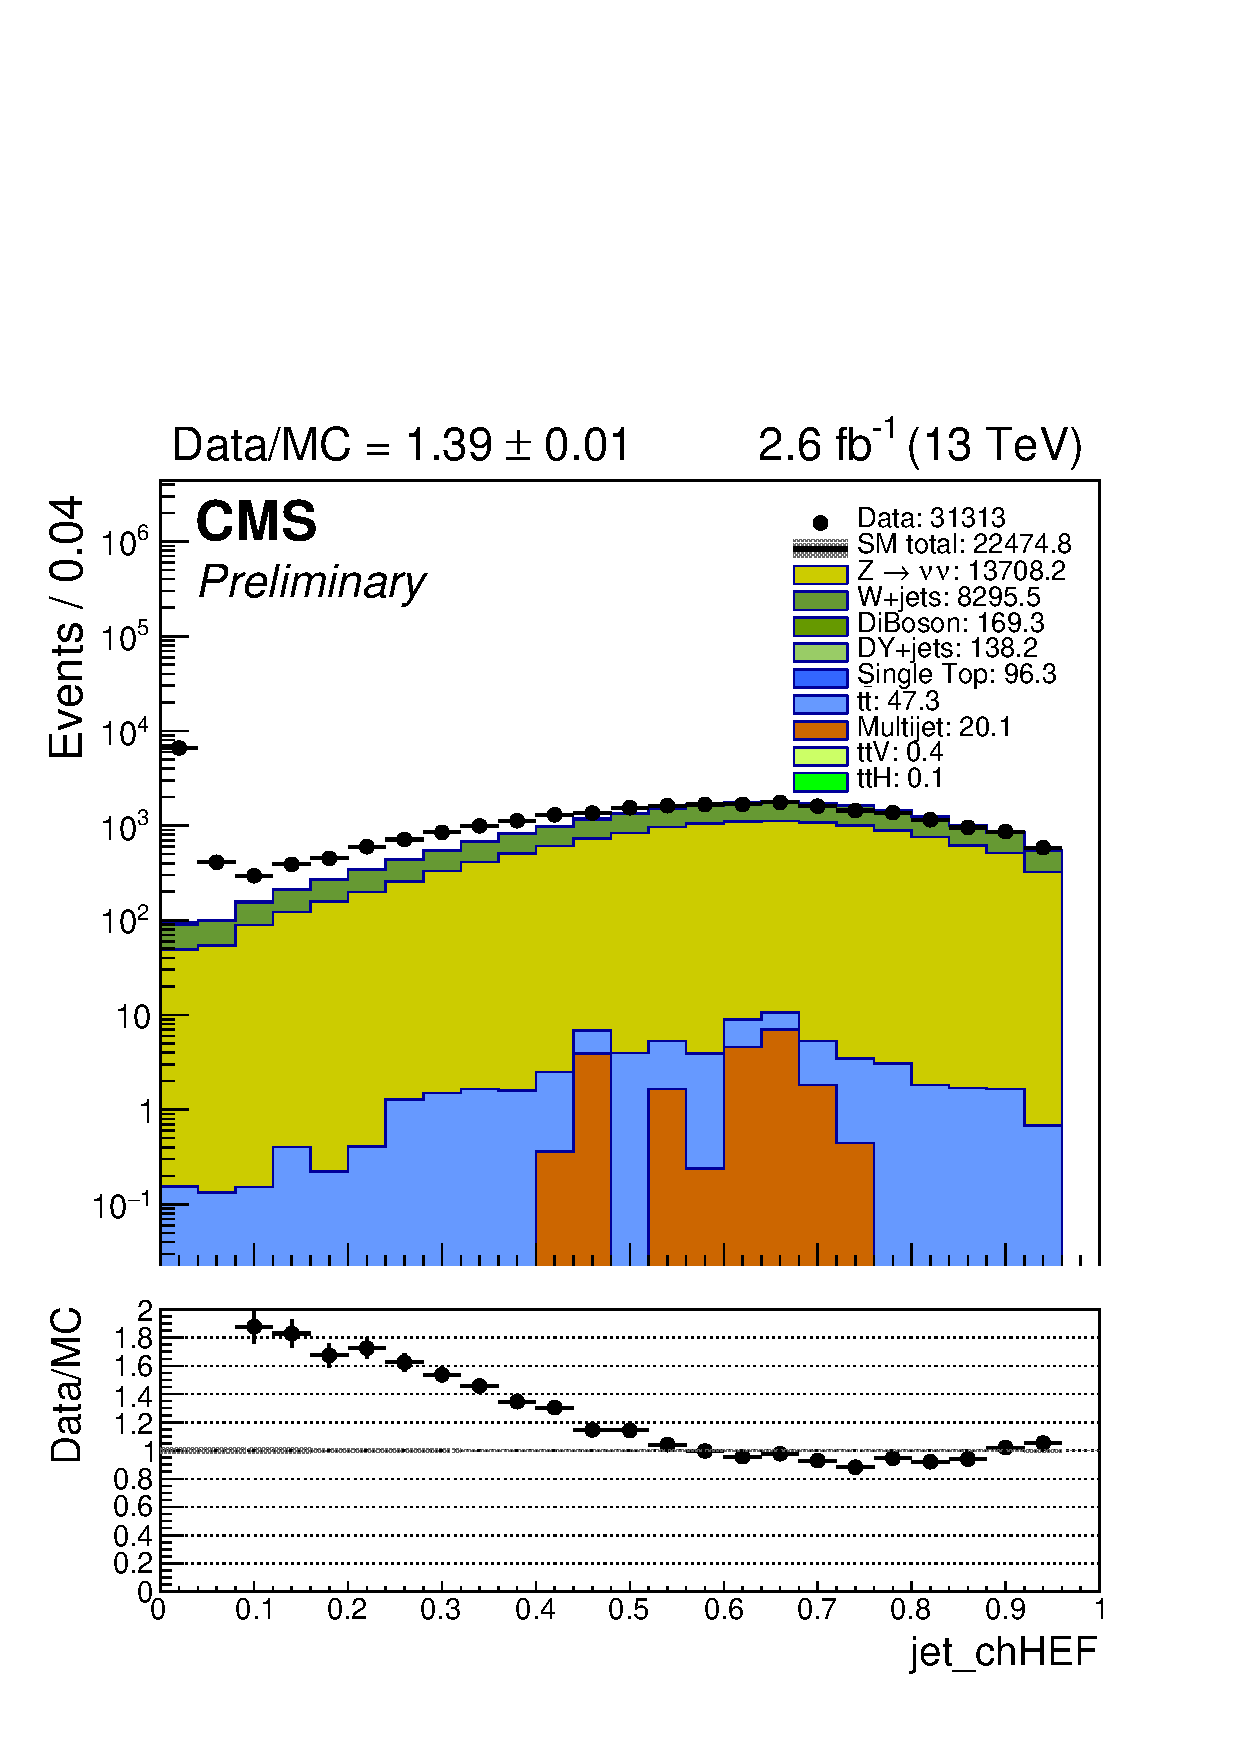
\includegraphics[width=0.32\textwidth]{figs/analysis/jet_chHEF_mono_all_before.pdf}
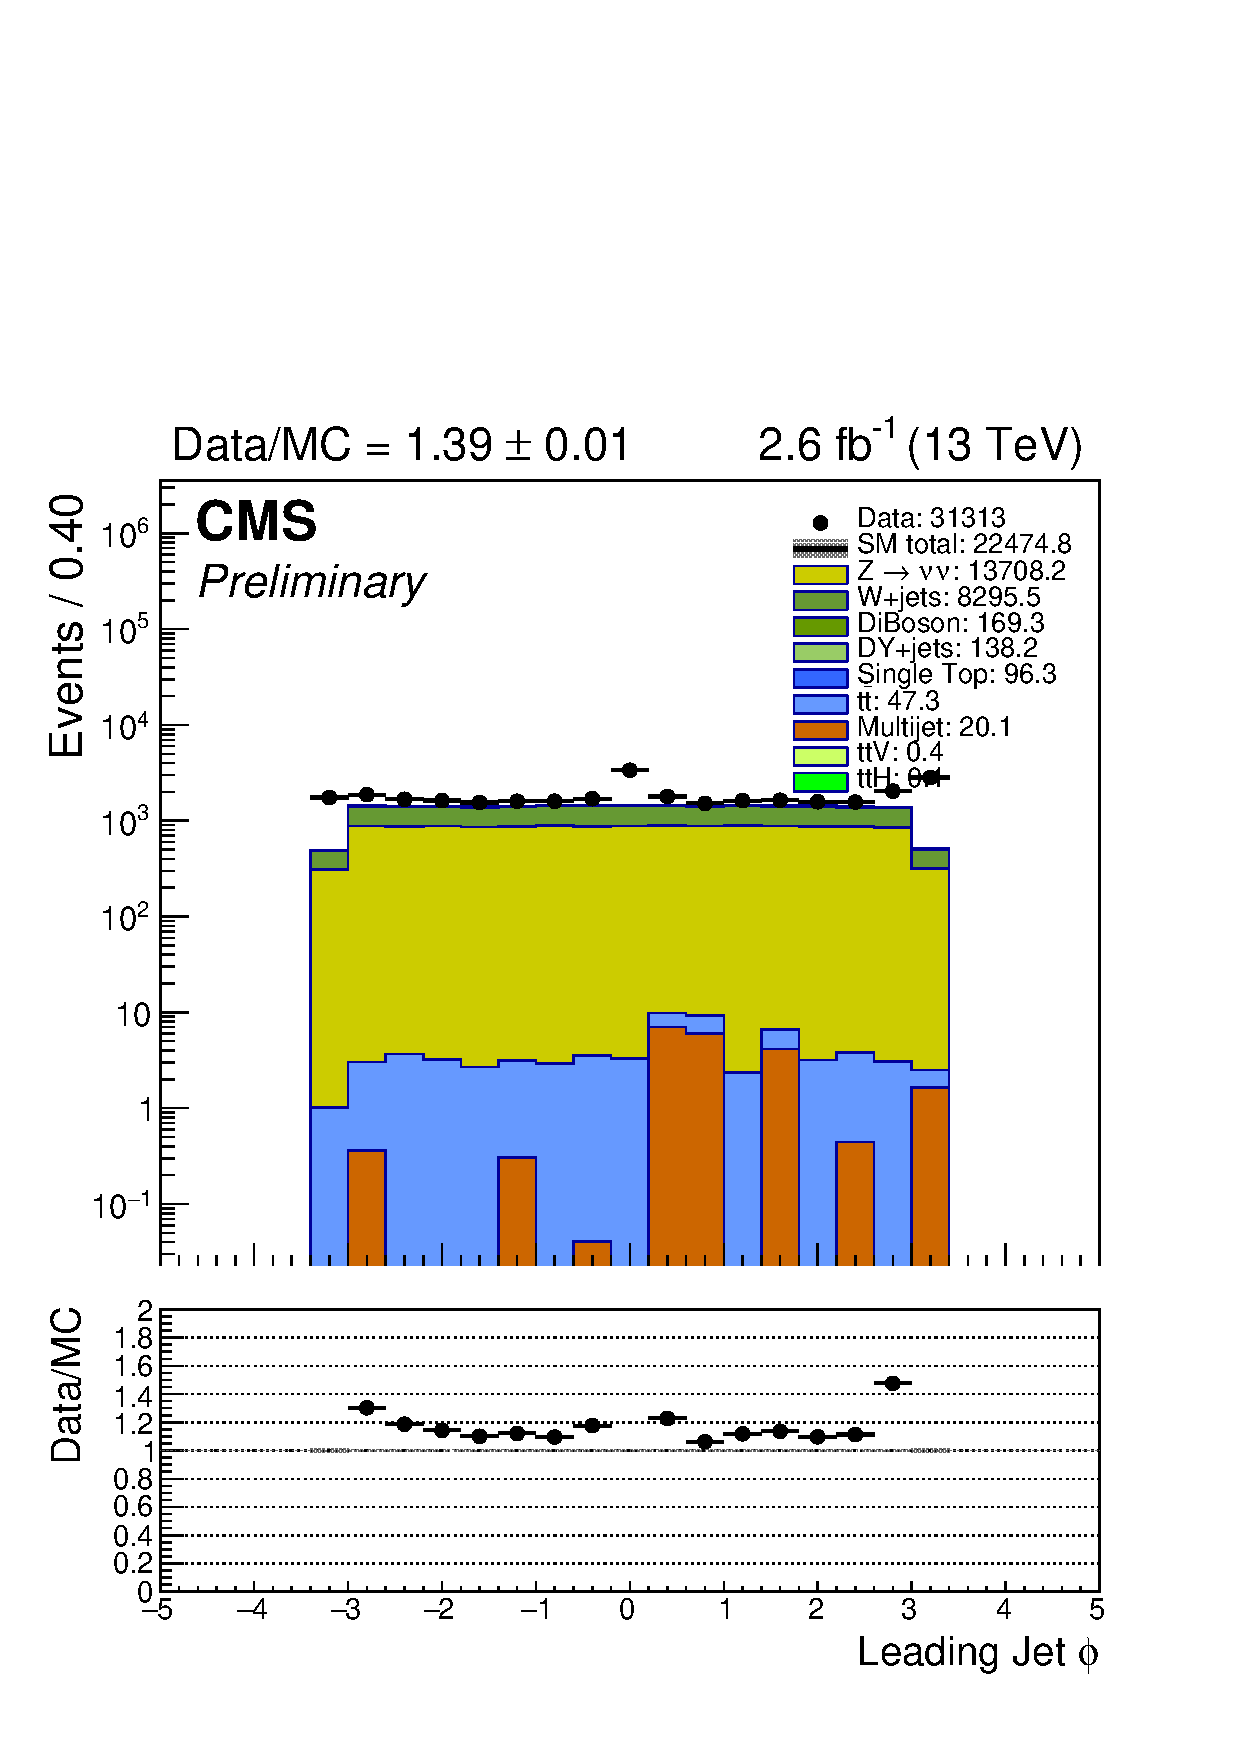
\includegraphics[width=0.32\textwidth]{figs/analysis/jet_phi[0]_mono_all_before.pdf}
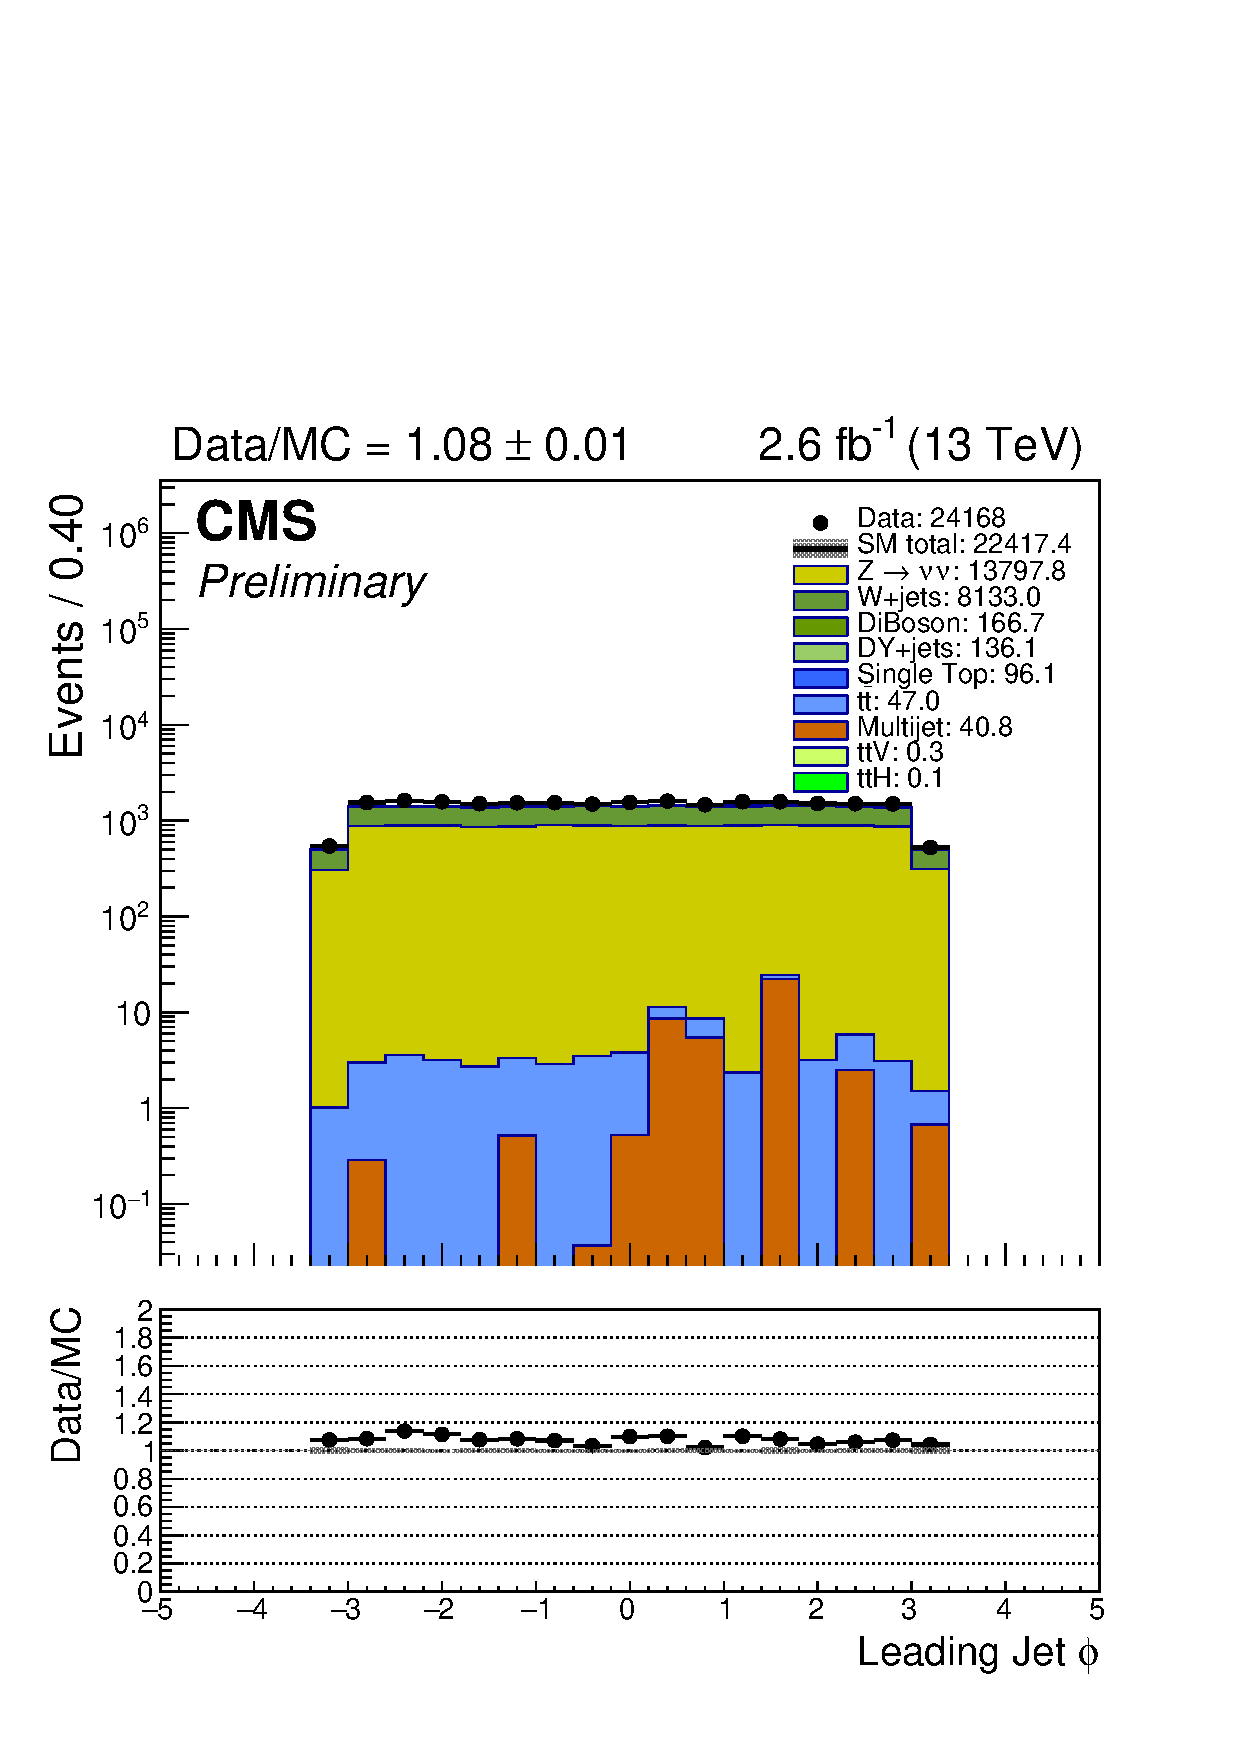
\includegraphics[width=0.32\textwidth]{figs/analysis/jet_phi[0]_mono_all_after.pdf}
\caption{The leading jet's charged hadron energy fraction (Left) and $\phi$ 
direction before (Centre) and after (Right) applying a requirement of 
\chf~$>0.1$. The large excess in data at \chf values close to zero and $\phi = 
0$ and $\pi$ is consistent with beam halo effects, and is effectively 
suppressed by the \chf requirement.}
\label{fig:beamhalo}
\end{center}
\end{figure}

%odd jet veto
As a further safeguard against noise and misreconstruction effects, events that 
contain a jet that fails the identification requirements outlined in 
Sec.~\ref{analysis-physicsobjects} are not considered.

%Forward jet veto here or QCD rejection? both
Finally within the set of baseline selections, events are vetoed if there are 
any jets with pseudorapidity direction \etaabs~$>2.4$. This threshold 
corresponds to the extent of the tracker and hence ensures well reconstructed 
jets and a better resolution of the energy sums. This requirement also has the 
added benefit of rejecting a larger proportion of background, particularly QCD 
processes, compared to signal processes, which tend to have more central 
jets.
%Adam: As most BSM physics scenarios result in the production of particles at a 
%high mass scale, they are more likely to deposit their energy centrally than 
%many of the SM backgrounds. Therefore, this forward jet veto does not 
%significantly effect the signal efficiency for most models. The QCD multijet 
%background consists of many soft scattering events, which typically deposit a 
%significant proportion of energy within the forward region

\section{Standard model backgrounds}
2-3 pages

After these requirements, still left with significant SM backgrounds from 
electroweak and QCD processes.

\subsection{Electroweak processes}

Dominant are Z and W.
	
Z is irreducible. Neutrinos.
	
W/ttbar is when lepton lost - not reconstructed or out of acceptance.
%or is produced in a direction that is not within the acceptance of the CMS 
%detector

Plus minor/residual backgrounds - single top, diboson, Higgs, etc.
	
\subsection{QCD processes}

Different QCD mechanisms (bullet list plus my studies) - detector effects, fake 
MET, mismeasurement, below threshold, heavy flavour.

\section{QCD background rejection}
2-3 pages.

Various ways of killing it: alphat, bdphi, mht/met.
Propaganda plots.

\subsection{alphaT}

\subsection{bdphi}

\subsection{missing energy ratio MHT/MET}

\section{Event selection}
2-3 pages

Now define the cuts to suppress the QCD, the definition of the signal region 
where we expect the signal, and the definition of the control regions that are 
used to estimate the SM backgrounds.

Big summary table of all selections/regions/objects (see paper).

define mono sym asym somewhere.

\subsection{Signal region}

alphat (summarise HT-dependent cuts in table), bdphi, mht/met cuts.
Anything else?

\subsection{Control regions}

Enriched in background they want to estimate. No overlap with SR events. 
Ignored lepton in sums to mimic/proxy the SR. Exactly the same cuts as SR 
except for inversion of muon veto to selection, plus some other differences 
described in the following.

Background estimation described in Sec X (EWK) and Y (QCD).

\subsubsection{mujets}

Exactly one muon that passes requirements mentioned before. DeltaR. MT. No 
alphat or bdphi.

\subsubsection{mumujets}

Exactly two muons opposite charge. DeltaR. Mll.

% \subsubsection{single photon}
% used in validation of nb, mHT?

\subsubsection{QCD sidebands} %hadronic control regions

bdphi and MHT/MET sidebands. Enriched in QCD.

\section{Event categorisation}
2 pages.

See AN.

Signal region binning in njet, nb, ht, mht. 
Jet pt (mono sym asym).

Same bins in single mu as SR.
Slightly different in double mu - only two nb bins. Explain why? Higher stats. 
Show nb extrapolation validation (AN) or just summarise briefly in couple of 
sentences (similar to MHT validation).

Table of bins.

%\subsection{Simplified binning scheme}
% Probably not necessary, just show results with nominal bins

%\subsection{Nb extrapolation}

\section{Triggers}
\label{sec:analysis-trigger}
5 pages.

See Mark.
List of SR and CR triggers.
Efficiencies.

\section{Simulation samples}
0.5 pages.
Maybe put here the "datasets" section of data and MC samples (see Matt).

\section{Corrections to simulation}
3-5 pages

Simulation modelling is not perfect. Need to correct it using scale factors by 
comparing data and MC. These corrections introduce systematic uncertainties in 
the background estimation, that will be described later in Sec X.

\subsection{Pileup}
\subsection{b-tagging efficiency}
Reweighting formula.
\subsection{Trigger efficiency}
\subsection{Lepton and photon reconstruction, identification, isolation and 
triggering efficiency}
Tag and probe.
\subsection{Top quark pT}
\subsection{Cross-sections}
Sideband corrections.
Summarise in table.

\subsection{Plus more?}
NLO, pdf/scale
Signal (maybe later): nISR, gen met

\section{b-tag formula method}
1-2 pages.

See Burton. AN Sec 4.4.
Relevant but be brief.
How much improves limits? Just refer to T1bbbb as T1qqqqLL 1 mm is very similar.

Purpose: reduce stat uncertainty of simulation in higher nb bins (where signal 
can lie).

Method: show the formula and explain it.

Summarise in table/plot or one-two sentences how much the stat unc is reduced. 
Maybe also how much the limits are improved (Lucien did this).

Formula systematics.
%\subsection{Systematics}

\section{Estimation of electroweak background processes}
Predict normalisation using CRs (data-driven to reduce reliance on MC). Use MHT 
templates from MC.

\subsection{nj, nb, ht dimensions}
1 page

Transfer factor method.

\subsection{MHT dimension}
2 pages

Take templates because don't want to bin CRs too finely (lose statistical power 
- curse of dimensionality).

Validation: Check data MC ratio is flat in CRs. Assign syst as described later 
in Sec X.

\section{Estimation of QCD background processes}
2 pages

Method.

Validation.

Plot of estimated yields per bin.

\section{Systematic uncertainties on background estimation}

These are explained below and also summarised, with representative magnitudes, 
in the big summary table of systs.

\subsection{MC-based}
3-4 pages (maybe 2 pages just of plots).

Known theoretical and experimental uncertainties.
Largely cancel out in the TF ratio.

Refer to Section of corrections to simulation. These are the associated 
uncertainties.

Pileup, JEC, b-tagging, lepton, photon, trigger, top pt, W/tt, NLO, ttbar nISR.

Example 2D plots of variations in the bins.

\subsection{Closure tests}
2-3 pages.

Probe additional sources of systematics.

Define method.

Go through each test (there's not many now) and describe what it's probing: 
extrapolation in alphat and bdphi, W polarisation, SITV.

Closure plots.

\subsection{MHT templates}
2 pages. See Matt and old ANs.

Derivation of uncertainties. Vs njet and ht.

Plot illustrating size of uncertainty in each bin.
